\section{支持BusyBox所需系统调用}
\subsection{编写面向POSIX标准的系统调用}
\subsubsection{支持BusyBox所需系统调用}

要从一个二进制文件中提取出相关的系统调用,需要经历如\ref{fig:pipe}所示的步骤:

\begin{figure}[htb]
    \centering
    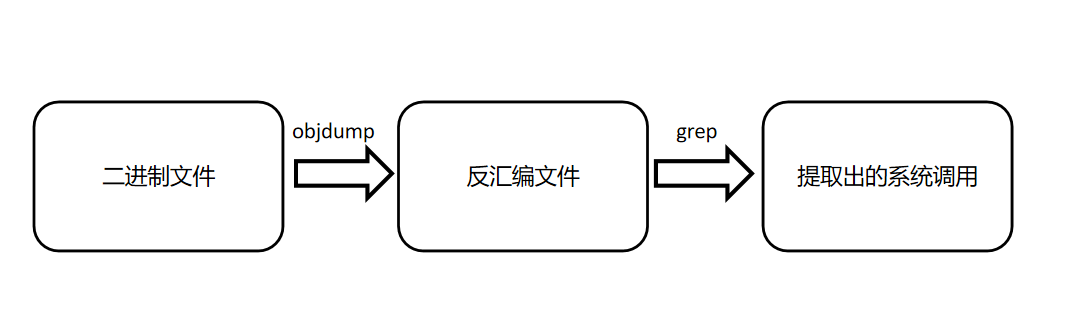
\includegraphics[width=\textwidth]{figures/09-03-系统调用抽取.png}
    \caption{
        从二进制文件中提取系统调用的的步骤
    }
    \label{fig:get_syscall}
\end{figure}

这些指令可以用一行命令完成。

\begin{lstlisting}[language=bash]
    # 从二进制文件中获取系统调用号,将objfile改为提取的目标二进制文件
    objdump -d objfile | grep -B 9 ecall | grep "li.a7" | tee syscall.txt

    # 如果报错:objdump: can't disassemble for architecture UNKNOWN! ,是由于当前的objdump并非RISC-V架构,尝试
    riscv64-linux-gnu-objdump -d busybox | grep -B 9 ecall | grep "li.a7" | tee syscall.txt

\end{lstlisting}

objdump -d objfile: 这部分使用objdump工具对目标文件(objfile)进行反汇编,显示其汇编代码。

grep -B 9 ecall: 这部分使用grep命令在反汇编的输出中查找包含字符串\enquote{ecall}的行,并显示该行及其前面的9行(-B 9选项)。

grep \enquote{li.a7}: 在前一步的输出中,再次使用grep命令查找包含字符串\enquote{li.a7}的行。

tee syscall.txt: 最后,将前两个grep命令的输出保存到一个名为syscall.txt的文件中,并在屏幕上显示这些输出。

上述三条命令通过管道连接,传递结果,加工完毕后存储到syscall.txt文本文件中。而要深入理解这些代码,我们首先要分析各个格式文件的具体内容。

二进制文件的汇编不再进行讲解。下面给出一个反汇编出的程序片段:

\begin{lstlisting}[language={[RISC-V]Assembler}]
    1062c:	0b953c27          	fsd	fs9,184(a0)
    10630:	0da53027          	fsd	fs10,192(a0)
    10634:	0db53427          	fsd	fs11,200(a0)
    10638:	4d3c506f          	j	0xd630a
    1063c:	08100893          	li	a7,129
    10640:	00000073          	ecall
    10644:	78fd                lui	a7,0xfffff
    10646:	00a8e363          	bltu	a7,a0,0x1064c
    1064a:	8082                ret
    1064c:	5880006f          	j	0x10bd4
    10650:	8082                ret
    10652:	0000                unimp
    10654:	0a000893          	li	a7,160
    10658:	00000073          	ecall
\end{lstlisting}

让我们结合汇编代码分析调用系统调用的一般结构。上面的代码中有两条ecall指令,ecall指令结合上面一行的 li a7, [系统调用号] 指令,即可实现特定系统调用的调用。在调用之前,还可能存在若干条指令,用于存入系统调用需要的参数。
比如,在调用64号write系统调用时,可能存在若干条li指令,将文件描述符、缓冲区指针、缓冲区长度分别写入a0、a1、a2寄存器中。

因此,当我们反汇编出如上格式的汇编代码时,为了提取出相关的系统调用,我们首先就要执行 grep -B 9 ecall 指令,将系统调用及前面的若干条指令提取出来。
为什么不直接提取 li a7, [系统调用号] ?这里的问题在于,a7并不是仅用于系统调用,有时也作为临时变量参与运算,因此,直接提取是不恰当的,将造成提取出的结果增多。
所以我们首先利用 grep -B 9 ecall 指令,把系统调用筛选出来,再获取其系统调用号。

当我们执行了 grep -B 9 ecall 后,获得到的汇编指令集合如下所示。

\begin{lstlisting}[language={[RISC-V]Assembler}]
--
  10a4d2:	26a73703          	ld	a4,618(a4) # 0x1bd738
  10a4d6:	40a006bb          	negw	a3,a0
  10a4da:	547d                li	s0,-1
  10a4dc:	9712                add	a4,a4,tp
  10a4de:	c314                sw	a3,0(a4)
  10a4e0:	b7e9                j	0x10a4aa
  10a4e2:	00b50b63          	beq	a0,a1,0x10a4f8
  10a4e6:	48e1                li	a7,24
  10a4e8:	4601                li	a2,0
  10a4ea:	00000073          	ecall
--
  10a51a:	000b3797          	auipc	a5,0xb3
  10a51e:	21e7b783          	ld	a5,542(a5) # 0x1bd738
  10a522:	40a0073b          	negw	a4,a0
  10a526:	557d                li	a0,-1
  10a528:	9792                add	a5,a5,tp
  10a52a:	c398                sw	a4,0(a5)
  10a52c:	8082                ret
  10a52e:	03b00893          	li	a7,59
  10a532:	4581                li	a1,0
  10a534:	00000073          	ecall
--
  10a5d8:	7dee                ld	s11,248(sp)
  10a5da:	8552                mv	a0,s4
  10a5dc:	7a52                ld	s4,304(sp)
  10a5de:	6135                addi	sp,sp,352
  10a5e0:	8082                ret
  10a5e2:	8a2a                mv	s4,a0
  10a5e4:	d161                beqz	a0,0x10a5a4
  10a5e6:	48c5                li	a7,17
  10a5e8:	8552                mv	a0,s4
  10a5ea:	00000073          	ecall
--
\end{lstlisting}

如此,就基本确保 li a7, 立即数 指令为系统调用时使用。此时再进行 grep \enquote{li.a7} ,就可以提取出所有系统调用号。最后的结果使用 tee syscall.txt 存入到 syscall.txt 中。
至此提取系统调用的命令的全过程也就清晰了。

\begin{figure}[h]
    \centering
    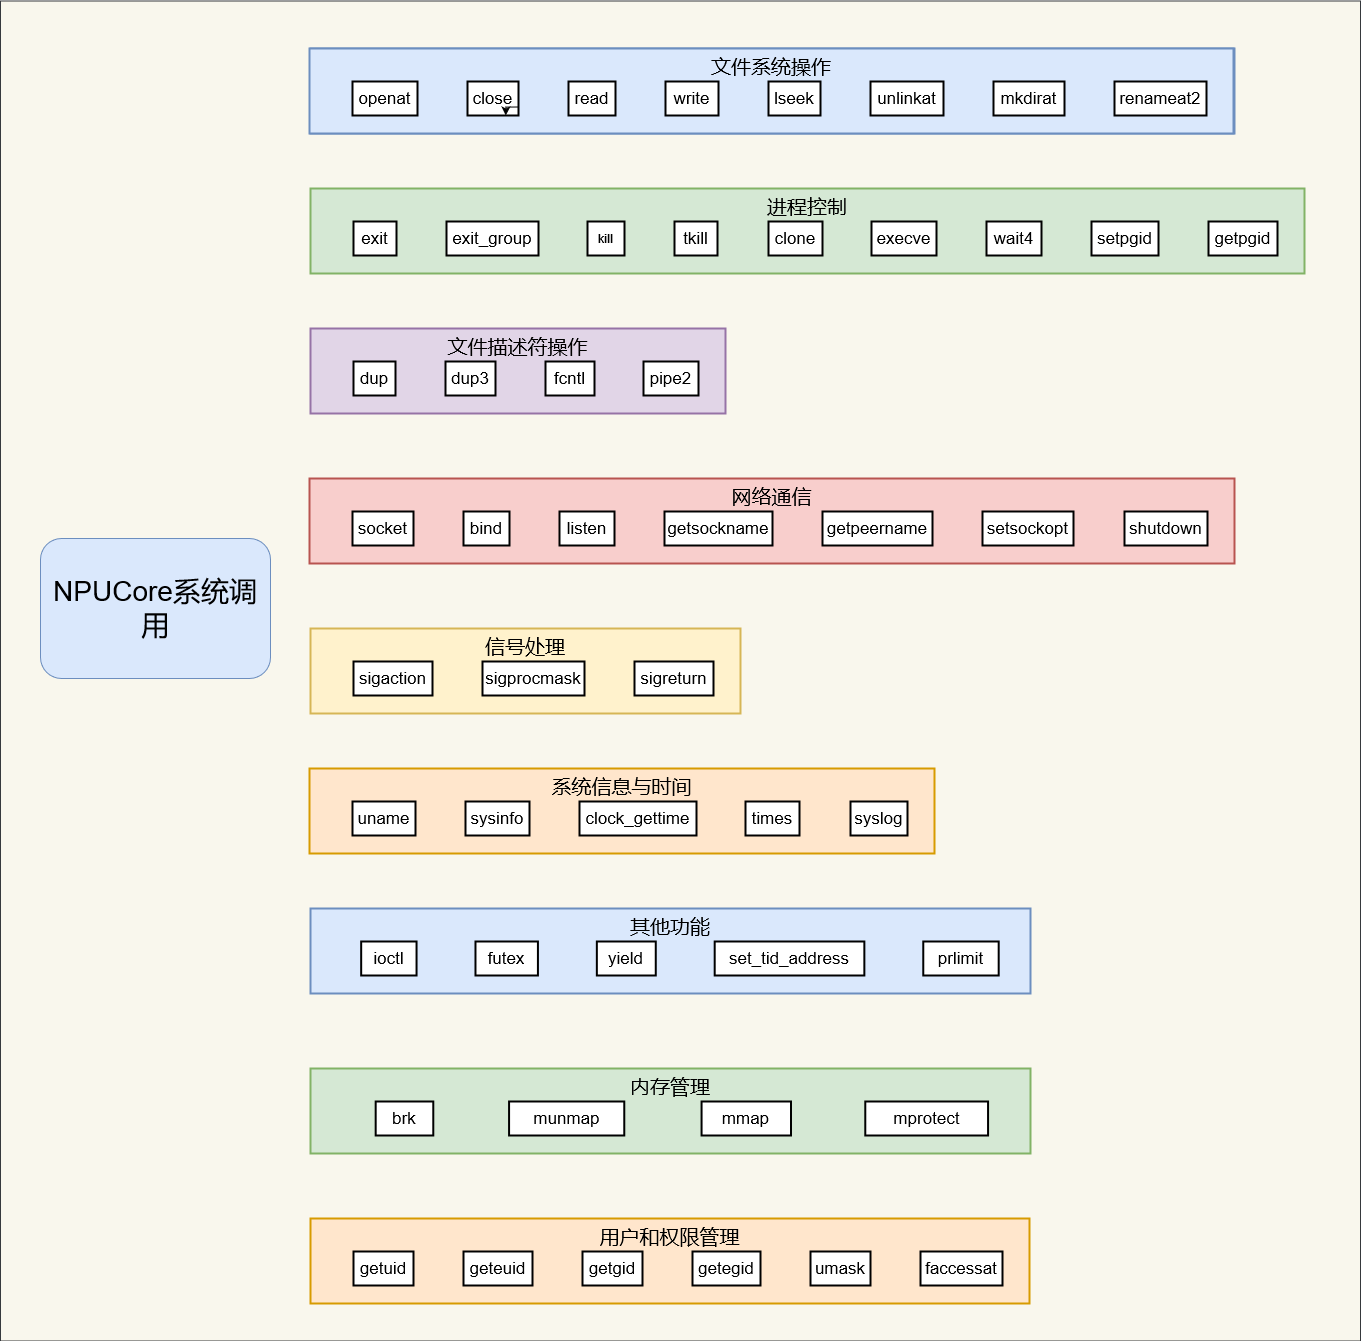
\includegraphics[width=0.7\textwidth]{figures/09-03-NPUCore系统调用.png}
    \caption{
        BusyBox系统调用
    }
    \label{fig:BusyBox系统调用}
\end{figure}
\subsection{BusyBox系统调用功能分类}
    
在本节中,我们将深入探讨BusyBox和NPUcore操作系统内核之间的系统调用交集。

首先,我们从BusyBox的系统调用列表开始,这个列表包含BusyBox运行所需的\textbf{\href{https://gitee.com/oscomp/testsuits-for-oskernel/blob/final-comp/docs/busybox_musl_static_syscall.txt}{各种系统调用}}。然后与NPUCore中的系统调用进行对照得到了一共\textbf{71}个系统调用。我们在进行对照的基础之上,对我们所得到的系统调用进行了分类,我们将其分为:

\begin{itemize}
  \item 文件系统操作
  \item 进程控制
  \item 信号处理
  \item 网络通信
  \item 文件描述符操作
  \item 系统信息与时间
  \item 用户和权限管理
  \item 内存管理
  \item 其他功能
\end{itemize}
接下来,我们将分类对每一类的部分系统调用进行介绍,在最后我们将给出所有系统调用与其功能的对应表。
\subsection{系统调用分类功能介绍}
\subsubsection*{文件系统操作}
文件系统操作涉及创建、打开、读取、写入、移动和删除文件或目录。
\begin{itemize}
    \item \textbf{openat}: 在指定目录下打开一个文件。
    \item \textbf{close}: 关闭一个已打开的文件描述符。
    \item \textbf{read}: 从打开的文件中读取数据。
    \item \textbf{write}: 向打开的文件写入数据。
    \item \textbf{lseek}: 在打开的文件中移动读写位置。
    \item \textbf{unlinkat}: 删除一个文件或目录链接。
    \item \textbf{mkdirat}: 在指定目录下创建一个新目录。
    \item \textbf{renameat2}: 重命名或移动一个文件或目录。
\end{itemize}
\subsubsection*{进程控制}
进程控制包括进程的创建、结束和信号处理。
\begin{itemize}
    \item \textbf{exit}: 结束调用它的进程。
    \item \textbf{exit\_group}: 结束与调用进程相同进程组的所有进程。
    \item \textbf{kill}: 向指定进程发送信号。
    \item \textbf{tkill}: 向指定线程发送信号。
    \item \textbf{clone}: 创建一个新进程,是 Linux 线程创建的基础。
    \item \textbf{execve}: 在当前进程中加载并运行一个新程序。
    \item \textbf{wait4}: 等待进程状态发生变化。
    \item \textbf{setpgid}: 设置进程组ID。
    \item \textbf{getpgid}: 获取指定进程的进程组ID。
\end{itemize}
\subsubsection{信号处理}
信号处理包括设置信号的处理方式、控制信号的屏蔽以及从信号处理程序返回。
\begin{itemize}
    \item \textbf{sigaction}: 设置信号的处理函数。
    \item \textbf{sigprocmask}: 用于阻塞或解除阻塞信号。
    \item \textbf{sigreturn}: 从信号处理程序返回。
\end{itemize}
\subsubsection{网络通信}
网络通信涉及套接字的创建、管理、绑定、监听及关闭。
\begin{itemize}
    \item \textbf{socket}: 创建一个新的套接字。
    \item \textbf{bind}: 将套接字绑定到一个地址。
    \item \textbf{listen}: 监听套接字连接。
    \item \textbf{getsockname}: 获取套接字的本地地址信息。
    \item \textbf{getpeername}: 获取远程连接端的地址信息。
    \item \textbf{setsockopt}: 设置套接字选项。
    \item \textbf{shutdown}: 关闭套接字的一部分或全部连接。
\end{itemize}
\subsubsection{文件描述符操作}
文件描述符操作涉及复制文件描述符、修改其属性及创建管道。
\begin{itemize}
    \item \textbf{dup}: 复制一个文件描述符。
    \item \textbf{dup3}: 复制文件描述符,提供额外的控制。
    \item \textbf{fcntl}: 对文件描述符进行各种控制操作。
    \item \textbf{pipe2}: 创建一个管道。
\end{itemize}
\subsubsection{系统信息与时间}
系统信息与时间包括获取系统和进程时间信息及生成系统日志。
\begin{itemize}
    \item \textbf{uname}: 获取系统信息。
    \item \textbf{sysinfo}: 获取系统统计信息。
    \item \textbf{clock\_gettime}: 获取当前时间。
    \item \textbf{times}: 获取进程时间信息。
    \item \textbf{syslog}: 生成系统日志消息。
\end{itemize}
\subsubsection{用户和权限管理}
用户和权限管理涉及获取用户/组ID、设置文件模式掩码及访问权限。
\begin{itemize}
    \item \textbf{getuid}: 获取用户ID。
    \item \textbf{geteuid}: 获取有效用户ID。
    \item \textbf{getgid}: 获取组ID。
    \item \textbf{getegid}: 获取有效组ID。
    \item \textbf{umask}: 设置文件模式创建掩码。
    \item \textbf{faccessat}: 检查文件的访问权限。
\end{itemize}
\subsubsection{内存管理}
内存管理包括数据段大小的调整、内存映射及内存保护。
\begin{itemize}
    \item \textbf{brk}: 改变数据段的大小。
    \item \textbf{munmap}: 取消内存映射。
    \item \textbf{mmap}: 映射文件或设备到内存。
    \item \textbf{mprotect}: 改变内存区域的保护权限。
\end{itemize}
\subsubsection{其他功能}
其他功能包括设备特定操作、线程管理等。
\begin{itemize}
    \item \textbf{ioctl}: 设备特定的输入/输出操作。
    \item \textbf{setsockopt}: 设置套接字选项。
    \item \textbf{futex}: 用户空间线程的快速锁机制。
    \item \textbf{yield}: 使当前线程放弃处理器。
    \item \textbf{set\_tid\_address}: 设置线程ID地址。
    \item \textbf{prlimit}: 获取和设置资源限制。
\end{itemize}
\subsubsection{系统调用功能对照表}
由于系统调用过多,我们在该部分仅用表格的形式将系统调用与其对应关系进行介绍。具体想要得到各个系统调用的细节,可以参考下一节中利用Linux man page命令得到。

\begin{table}[h]
\centering
\begin{tabular}{|c|c|c|c|c|c|}
\hline
\textbf{调用} & \textbf{描述} & \textbf{调用} & \textbf{描述} & \textbf{调用} & \textbf{描述} \\
\hline
dup & 文件描述符复制 & dup3 & 类似dup但可设置标志 & getcwd & 获取当前目录路径 \\
fcntl & 文件描述符操作 & ioctl & 设备控制 & mkdirat & 创建新目录 \\
unlinkat & 删除文件 & linkat & 创建硬链接 & umount2 & 卸载文件系统 \\
mount & 挂载文件系统 & faccessat & 检查文件权限 & chdir & 更改目录 \\
openat & 打开文件 & close & 关闭文件描述符 & pipe2 & 创建管道 \\
getdents64 & 读取目录项 & lseek & 文件定位 & read & 读取数据 \\
write & 写入数据 & readv & 多缓冲区读取 & writev & 多缓冲区写入 \\
sendfile & 传输数据 & ppoll & 等待事件 & readlinkat & 读取链接 \\
fstatat & 文件状态 & fstat & 描述符状态 & statfs & 文件系统状态 \\
ftruncate & 截断文件 & utimensat & 设置时间戳 & exit & 终止进程 \\
exit\_group & 终止进程组 & set\_tid\_address & 设置线程ID & futex & 锁定机制 \\
setitimer & 定时器 & clock\_gettime & 获取时间 & syslog & 内核缓冲操作 \\
yield & 让出时间 & kill & 发送信号 & tkill & 向线程发送信号 \\
sigaction & 信号处理 & sigprocmask & 信号集更改 & sigreturn & 返回信号处理 \\
times & 进程时间 & setpgid & 设置进程组ID & getpgid & 获取进程组ID \\
uname & 系统信息 & umask & 文件模式掩码 & getpid & 获取进程ID \\
getppid & 获取父进程ID & getuid & 获取用户ID & geteuid & 获取有效用户ID \\
getgid & 获取组ID & getegid & 获取有效组ID & gettid & 获取线程ID \\
sysinfo & 系统信息 & socket & 创建套接字 & bind & 绑定地址 \\
listen & 监听连接 & getsockname & 套接字信息 & getpeername & 端点地址 \\
setsockopt & 套接字选项 & brk & 数据段分配 & munmap & 解除映射 \\
clone & 创建子进程 & execve & 执行程序 & mmap & 映射内存 \\
mprotect & 内存权限 & wait4 & 等待状态变化 & prlimit & 资源限制 \\
renameat2 & 重命名 & shutdown & 关闭连接 & & \\
\hline
\end{tabular}
\caption{NPUCore系统调用及其功能}
\label{table:syscallscompact}
\end{table}
\subsection{获取系统调用相关信息}
Posix规范规定了一系列的系统调用,linux提供了查看系统调用相关信息的命令,如下所示:
\begin{lstlisting}[language=bash]
    man 2 open 
\end{lstlisting}
可以查看open系统调用的相关信息,如下所示:
\begin{figure}[H]
  \centering
  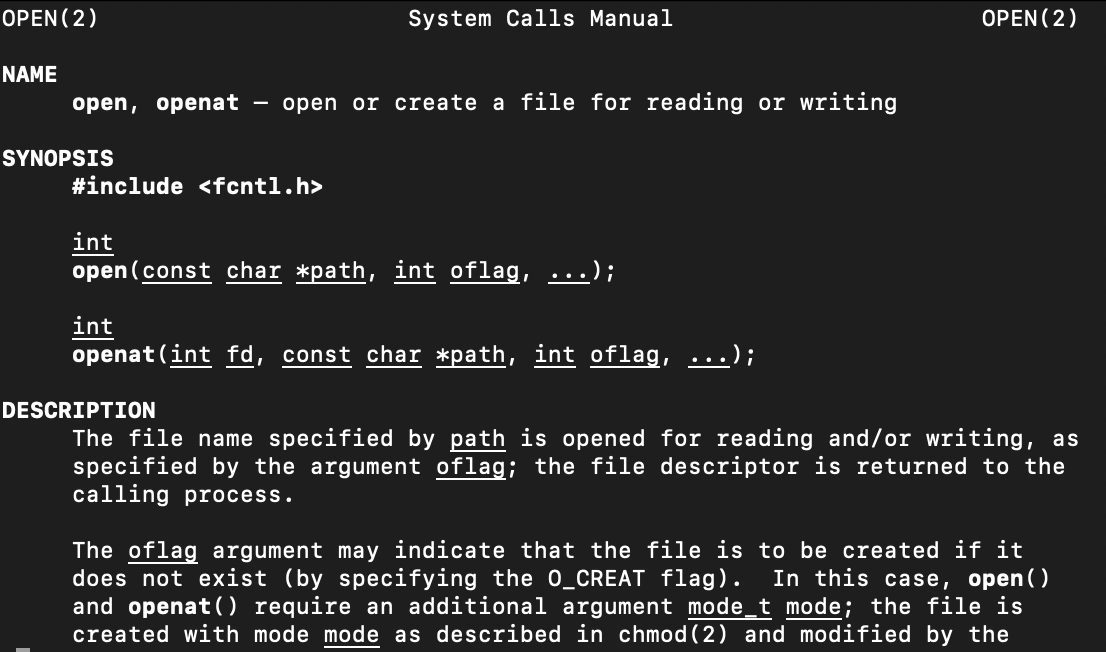
\includegraphics[width=0.8\textwidth]{figures/09-03-open系统调用manu信息.png}
  \caption{open系统调用相关信息}
  \label{fig:opensyscall}
\end{figure}
每个man指令的手册页面都有类似的结构,由以下部分组成
\begin{itemize}
    \item NAME:命令的名称和简短描述
    \item SYNOPSIS:命令的语法和选项 初步描述了命令的基本用法
    \item DESCRIPTION:命令的详细描述和用法
    \item OPTIONS:命令的选项和参数
    \item EXAMPLES:使用命令的示例
    \item FILES:命令可能使用的文件
    \item SEE ALSO:相关命令和手册页面
    \item BUGS:已知的命令错误和限制
    \item AUTHOR:命令的作者和贡献者
\end{itemize}
man是系统的分页(page)手册,指定的man的页选项通常是程序工具或函数名,程序将显示每一项找得到的相关手册页。
如果指定了章节(section),man将在指定章节中搜索。
默认将按照预定的顺序查找所有可用的章节,并且只显示第一个页,即使在多个章节中都存在这个页。
可以在\ref{fig:opensyscall}看到,在man页面的左上角,有一个MAN(2),这里的2就是章节,比较常用的章节号是1、5、8,分别代表用户命令、配置文件和格式、系统管理命令。

通过在文档中找到我们想要的规范信息,我们可以知道实现系统调用的细节规范,如报错类型,返回类型,接口参数等。

接下来,我们以open系统调用为例,来看看如何实现系统调用。
第一步,需要从linux man page中找到open系统调用的系统调用号和函数签名,并将其如\ref{fig:opensyscall1}所示:
\begin{figure}[H]
  \centering
  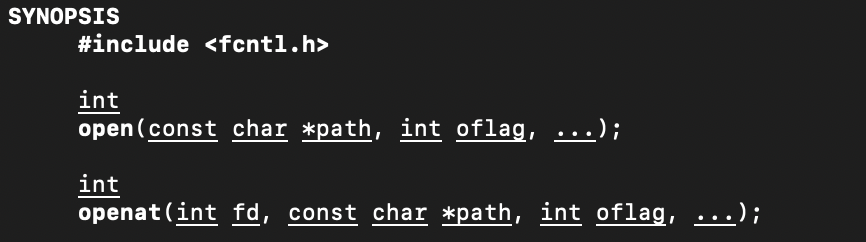
\includegraphics[width=0.8\textwidth]{figures/09-03-open系统调用签名.png}
  \caption{open系统调用号和函数签名}
  \label{fig:opensyscall1}
\end{figure}

第二步,分析该系统调用设计的模块,具体而言是需要实现的功能与内核的哪一个部分关联,例如内存映射、进程管理、进程通信、线程相关等。
之后,分析具体实现的框架,也就是做那些操作,我们需要的函数接口是哪些,从而可以得出一个实现的伪代码。
在open的例子中,我们可以得到如下的伪代码:
\begin{lstlisting}[language=c]
    int open(const char *pathname, int flags, mode_t mode)
    {
        // 1. 检查参数是否合法
        // 2. 从文件系统中找到文件
        // 3. 根据flags和mode参数,检查文件是否可以打开
        // 4. 为文件分配一个文件描述符
        // 5. 返回文件描述符
    }
\end{lstlisting}

最后,在代码实现上,关注手册中的细节,例如可能出现的错误信息,对于特殊情况的处理。
如在open的例子中,可能出现的错误类型有:
\begin{itemize}
    \item EACCES:文件不可访问
    \item EEXIST:文件已经存在
    \item EFAULT:pathname指向的内存空间不可访问
    \item EINTR:调用被信号中断
    \item EISDIR:pathname指向的是一个目录
    \item ELOOP:pathname指向的是一个循环链接
    \item EMFILE:进程打开的文件数超过了系统限制
    \item ENAMETOOLONG:pathname太长
    \item ENFILE:系统打开的文件数超过了系统限制
    \item ENODEV:pathname指向的文件不存在
    \item ENOENT:pathname指向的文件不存在
    \item ENOMEM:内存不足
    \item ENOTDIR:pathname指向的不是一个目录
    \item ENXIO:pathname指向的设备不存在
    \item EOVERFLOW:文件太大
    \item EPERM:pathname指向的文件不可访问
    \item EROFS:pathname指向的文件是只读的
    \item ETXTBSY:pathname指向的文件正在被使用
    \item EWOULDBLOCK:O\_NONBLOCK被设置,但是文件被阻塞
\end{itemize}

如此,我们就完整的实现了一个系统调用。类似的对于其他的系统调用,我们都可以类似的实现。